\section{EXPERIMENTS}

% Dataset description
\paragraph{Datasets}
We evaluate our GP-RFM-Laplace on a variety of regression tasks.
Specifically, we use two tabular regression benchmarks with datasets from UCI \citep{asuncion2007uci} and OpenML \citep{vanschoren2014openml} respectively.
For the UCI benchmark we use 7 datasets inspired by \citet{duan2020ngboost} and
for the OpenML benchmark, we utilize the collection of 16 numerical regression datasets by \citet{grinsztajn2022tree}.

% Hyperparameter tuning and preprocessing
\paragraph{Hyperparameter tuning}
We follow the protocol proposed in \citet{hernandez2015probabilistic} for data splitting and hyperparameter tuning.
For the UCI benchmark, we follow \citet{duan2020ngboost} to hold out 10\% of the data as a test set.
For the OpenML benchmark, we follow \citet{grinsztajn2022tree} to hold out 30\% of the data as a test set.
The remaining data is split into a 70\% training set and a 30\% validation set in order to tune the hyperparameters.
We use grid-search over all combinations of hyperparameters and select the best hyperparameters based on the NLL on the validation set.
Details on the hyperparameter search space can be found in the appendix.
Finally, we train the model on the full training set and evaluate it on the test set.
The process is repeated for 20 random seeds and we report the mean and standard deviation of the results.

% Baseline methods
\paragraph{Baselines}
%\begin{itemize}
%    \item GPs: RBF, Laplace, ARD-RBF, ARD-Laplace
%    \item Boosting: NGBoost, CatBoost-Ensemble
%\end{itemize}
We compare our GP-RFM-Laplace to a variety of probabilistic baseline methods.
For GPs, we consider the \emph{RBF} and \emph{Laplace} kernel.
% where we learn the length scale parameter $\ell$ and the noise variance $\sigma$.
Additionally, we compare to the \emph{ARD-RBF} \citep{neal1996bayesian} which is used in many settings and to the \emph{ARD-Laplace} kernel.
% where we learn the length scale parameters $\ell_1,\dots,\ell_d$ and the noise variance $\sigma$.
The latter is a rarely used kernel in GPs but is a natural extension of the Laplace kernel to incorporate feature weighting, learnt through NLL minimization.
% boosting approaches
% NGBoost generalizes gradient boosting to probabilistic regression by treating the parameters of the conditional distribution as targets for a multiparameter boosting algorithm
Furthermore, we consider probabilistic extensions of boosting approaches, which are known to be powerful for predictive tasks.
Firstly, we use \emph{NGBoost} \citep{duan2020ngboost} which learns the parameters of a Gaussian distribution through boosting enhanced with a natural gradient update.
Secondly, we use \emph{CatBoost-Ensemble} \citep{prokhorenkova2018catboost} which uses an ensemble of 10 gradient boosting-based models from which the predictive distribution is obtained by computing statistics of the individual predictions.
% preprocessing
Following \citet{duan2020ngboost}, we standardize features and labels to have zero mean and unit variance for all GP-based methods but not for the boosting-based methods.



% Evaluation metrics
\paragraph{Evaluation metrics}
% RMSE, NLL, 95\% Coverage Error, Interval Length at 95\% Coverage
We are interested in the predictive performance of the models as well as their uncertainty quantification.
Therefore, we evaluate the models on their \emph{root mean squared error (RMSE)} as well as their \emph{NLL} on the test set.
We also require the model uncertainty to be calibrated, i.e. the predictive distribution should reflect the likelihood of prediction errors.
To evaluate calibration, we compute the \emph{95\% coverage error (CE)} which refers to the proportion of data points for which the 95\% prediction interval does not contain the true value.
In order for the model to be well-calibrated, the coverage should be 95\% and the corresponding CE should be zero.
Finally, we evaluate the \emph{interval length (IL)} of the 95\% confidence interval. This measure is important for models with similar CE since a smaller IL indicates a more precise uncertainty quantification.








\subsection{Main results}
Here we present the main results of our experiments.
We compare our GP-RFM-Laplace to all baseline methods on the UCI and OpenML benchmark datasets.
% normalization as datasets have different scales
Since the datasets have different scales, we normalize the resulting metrics to compare methods across datasets.
Specifically, for each dataset, we compute the minimum and maximum of the results across all methods and seeds.
Then, we normalize the results of each method and seed to the range $[0,1]$.
% results reference to figures and tables
The results for the OpenML benchmark are shown in \Cref{fig:main-tabular-benchmark} for NLL, RMSE and CE
using violin plots to show the distribution of the results including a boxplot for the median and quartiles.
The results for the UCI benchmark are shown in the appendix.
Note that the results for IL are omitted as comparing IL across datasets is not meaningful.
Detailed results for each dataset individually can be found in the appendix.

% results summary
We observe that our GP-RFM-Laplace is only outperformed by the CatBoost-Ensemble in terms of NLL.
However, the GP-RFM-Laplace is the best method in terms of RMSE, closely followed by the GP-ARD-Laplace.
Regarding calibration, we observe that the boosting methods are dominant, followed by the GP-RFM-Laplace.
Overall, both the GP-RFM-Laplace and the GP-ARD-Laplace perform similarly well across all metrics, demonstrating a competitive approach to boosting-based approaches for probabilistic regression.


\begin{figure}[htb]
    \centering
    \begin{subfigure}[b]{0.475\textwidth}
        \centering
        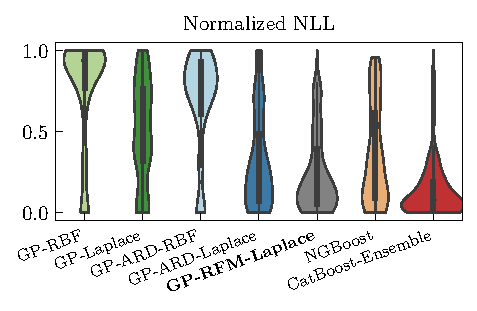
\includegraphics[trim=0 40 0 0, clip, width=\textwidth]{figures/tabularbenchmark_nll.pdf}
    \end{subfigure}
    % \hfill
    \begin{subfigure}[b]{0.475\textwidth}
        \centering
        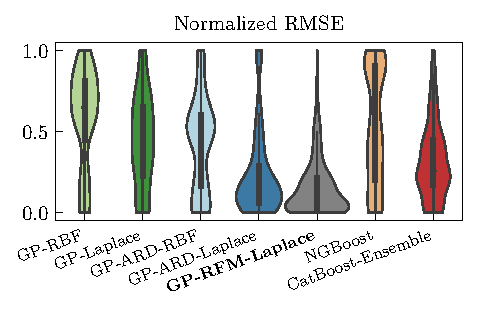
\includegraphics[trim=0 40 0 0, clip, width=\textwidth]{figures/tabularbenchmark_rmse.pdf}
    \end{subfigure}
    % \vskip\baselineskip
    \begin{subfigure}[b]{0.475\textwidth}
        \centering
        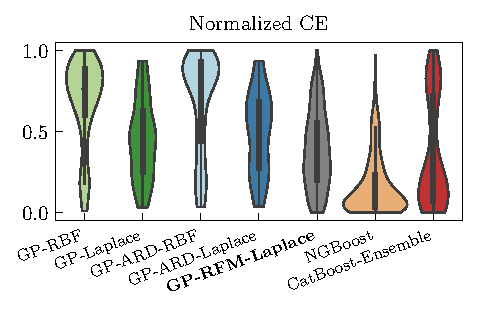
\includegraphics[width=\textwidth]{figures/tabularbenchmark_coverage.pdf}
    \end{subfigure}
    \caption{Violin plot results on OpenML benchmark datasets.}
    \label{fig:main-tabular-benchmark}
\end{figure}

% \daniel{plot of interval len rank vs coverage}








\subsection{Toy data set}
Given the qualitatively similar performance of the GP-RFM-Laplace and the GP-ARD-Laplace, we investigate the differences between the two methods in more detail.
Mathematically, the ARD kernel is equivalent to the RFM kernel with a diagonal feature matrix, learnt through NLL minimization instead of AGOP iterations.
Therefore, the RFM kernel can be seen as a generalization of the ARD kernel which can capture feature correlations which are relevant for the predictive task.

To highlight the difference between both kernels, we generate a toy dataset
where the features are independent $\vx\sim\gN(0,\mI_d)$ and the labels are the squared sum of the first 10 features $y=(\sum_{i=1}^{10} \vx_{[i]})^2$.
This dataset is designed to be challenging for the ARD kernel as it requires learning the feature correlation.
We compare the performance for a range of feature sizes in \Cref{fig:toy-data-nll}; the respective results for RMSE can be found in the appendix.

We observe that the GP-RFM-Laplace outperforms the GP-ARD-Laplace for all feature sizes.
Therefore, we conjecture that in the real-world datasets which we consider, there is either little feature correlation or the feature correlation is not relevant for the predictive task.
For datasets where the GP-RFM-Laplace considerably outperforms the GP-ARD-Laplace, such as the ISOLET (Isolated Letter Speech Recognition) dataset from OpenML, we observe that there is indeed considerable feature correlation.

\begin{figure}
    \centering
    % \includegraphics{figuresTikz/toy_data_nll}
    % \tikzsetnextfilename{toy_data_nll}
    \begin{tikzpicture}[baseline]

\pgfplotstableread[col sep=comma]{./data/toy_data_metrics.csv}{\datatable};
\begin{axis}[
width=\columnwidth,
height=.7\columnwidth,
ylabel={NLL},
xlabel={features $d$},
title={Toy data with feature correlation},
xmin=19,
xmax=131,
% ymin=0,
% ymax=0.5,
legend style={font=\tiny, 
	fill opacity=0.6, text opacity =1,
        at={(0.98,.18)},anchor=south east,
        row sep=-3pt,
        },
legend cell align={left},
% ytick={0, 0.08}, % Define the desired y tick positions
xtick={10, 30, 50, 70, 90, 110, 130}, % Define the desired y tick positions
yticklabel style={
	% /pgf/number format/fixed, % Use fixed point notation
	% /pgf/number format/precision=2, % Set the number of decimal places
	% /pgf/number format/fixed zerofill, % Fill in trailing zeros
        },
% ymode=log,
]


% RFM full
\addplot+ [black, 
mark=*,
mark options={solid},
% mark size=5pt,
thick,
error bars/.cd,
x dir=both,x explicit,
y dir=both,y explicit,
error bar style={solid}
]
table[x=features,y=GP_RFM_Laplace_full_NLPD_mean,y error=GP_RFM_Laplace_full_NLPD_std] {\datatable};

% % RFM diag
% \addplot+ [red, mark=x, mark size=5pt, thick,
% error bars/.cd,
% x dir=both,x explicit,
% y dir=both,y explicit,
% error bar style={solid}
% ]
% table[x=features,y=GP_RFM_Laplace_diag_NLPD_mean,y error=GP_RFM_Laplace_diag_NLPD_std] {\datatable};

% Laplace
\addplot+ [darkgreen, 
mark=*,
mark options={solid},
% mark size=5pt, 
thick,
error bars/.cd,
x dir=both,x explicit,
y dir=both,y explicit,
error bar style={solid}
]
table[x=features,y=GP_Laplace_NLPD_mean,y error=GP_Laplace_NLPD_std] {\datatable};

% ARD-Laplace
\addplot+ [darkblue, 
dotted,
mark=*,
mark options={solid},
% mark size=5pt, 
thick,
error bars/.cd,
x dir=both,x explicit,
y dir=both,y explicit,
error bar style={solid}
]
table[x=features,y=GP_ARD_Laplace_NLPD_mean,y error=GP_ARD_Laplace_NLPD_std] {\datatable};

% NG-boost
\addplot+ [orange,
dashed,
mark=*,
mark options={solid},
% mark size=5pt,
thick,
error bars/.cd,
x dir=both,x explicit,
y dir=both,y explicit,
error bar style={solid}
]
table[x=features,y=NG_Boost_NLPD_mean,y error=NG_Boost_NLPD_std] {\datatable};

% Cat-Boost Ensemble
\addplot+ [red, 
dashed,
mark=*,
mark options={solid},
% mark size=5pt, 
thick,
error bars/.cd,
x dir=both,x explicit,
y dir=both,y explicit,
error bar style={solid}
]
table[x=features,y=Cat_Boost_Ensemble_NLPD_mean,y error=Cat_Boost_Ensemble_NLPD_std] {\datatable};



\legend{
    {GP-RFM},
    {GP-Laplace}, 
    % {GP-RFM-diag},
    {GP-ARD-Laplace},
    {NGBoost},
    {CatBoost Ens.}
}

\end{axis}
\end{tikzpicture}
    \caption{Toy dataset with relevant feature correlation for prediction. We scale the number of train samples with $n=20 d$.}
    \label{fig:toy-data-nll}
\end{figure}








\subsection{Comparative feature evaluation}
Given the comparable performance of the GP-RFM-Laplace and the GP-ARD-Laplace, a second question arises regarding the learned features.
To investigate this, we compare the correlation between the diagonal of the feature matrix of the GP-RFM-Laplace and the GP-ARD-Laplace.
Additionally, we train a GP-RFM-Laplace where we restrict the feature matrix $\mM$ to be diagonal, i.e. we use the RFM-diag kernel.

\Cref{fig:feature-correlation} shows the correlation between the diagonal of the feature matrix for all three methods on the UCI benchmark datasets.
While there is a high correlation between all three methods for some datasets, there are also datasets where the correlation is low--even between the methods learning diagonal features, the RFM-diag and the GP-ARD-Laplace.
This indicates that learning the features with AGOP in the RFM or with NLL minimization in the ARD kernel
may result in the same features in some cases but is not guaranteed to do so.
Further investigation is required to understand the differences between feature learning in the two methods.


\begin{figure}
    \centering
    % \includegraphics{figuresTikz/feature_correlation}
    % \tikzsetnextfilename{feature_correlation}
    \begin{tikzpicture}
\pgfplotstableread[col sep=comma]{./data/correlation_rfmfull_rfmdiag.csv}{\datatableA};
\pgfplotstableread[col sep=comma]{./data/correlation_rfmfull_ard.csv}{\datatableB};
\pgfplotstableread[col sep=comma]{./data/correlation_rfmdiag_ard.csv}{\datatableC};
\begin{axis}[
boxplot/draw direction=y,
title={Feature correlation},
width=\columnwidth,
height=0.7\columnwidth,
boxplot={
	%
	% Idea: 
	%  place the 
	%  group 1 at 0.25 and 0.5 and 0.75
	%  group 2 at 1.25 and 1.5 and 1.75
	%  group 3 at 2.25 and 2.5 and 2.75
	%  ...
	% in a formular:
%	draw position={0.25 + floor(\plotnumofactualtype/3) + 0.25*mod(\plotnumofactualtype,3)},
	draw position={0.25 + floor(\plotnumofactualtype/3) + 0.25*mod(\plotnumofactualtype,3)},
	%
	% that means the box extend must be at most 0.2 :
	box extend=0.2,
},
% ... it also means that 1 unit in x controls the width:
%x=1.5cm,
xtick={0,1,2,...,8},
%xtick={0.5,1.5,2.5,3.5,4.5,5.5,6.5}
x tick label as interval,
xticklabels={%
	{YaHy},%
	{Ki},%
	{CoCoSt},%
	{CoCyPoPl},%
	{EnEf},%
	{NaPlMa},%
	{WiQuRe},%
},
xticklabel style={rotate=45, anchor=east}, % Rotate labels by 45 degrees
xmin=0,
xmax=7,
ymax=1.1,
ymin=-0.75,
legend style={font=\tiny, 
	fill opacity=0.9, text opacity=1,
	at={(0.02,0.02)},
	anchor=south west,
	row sep=0pt},
legend cell align={left},
area legend,
legend entries = {
	{RFM vs RFM-diag},
	{RFM vs ARD-Laplace},
	{RFM-diag vs ARD-Laplace},
},
]

%YaHy
\addplot[boxplot, thick, draw=darkblue] table[y index=6] {\datatableA};
\addplot[boxplot, thick, draw=darkgreen] table[y index=6] {\datatableC};
\addplot[boxplot, thick, draw=red] table[y index=6] {\datatableC};

%Ki
\addplot[boxplot, thick, draw=darkblue] table[y index=2] {\datatableA};
\addplot[boxplot, thick, draw=darkgreen] table[y index=2] {\datatableB};
\addplot[boxplot, thick, draw=red] table[y index=2] {\datatableC};

% CoCoSt
\addplot[boxplot, thick, draw=darkblue] table[y index=0] {\datatableA};
\addplot[boxplot, thick, draw=darkgreen] table[y index=0] {\datatableB};
\addplot[boxplot, thick, draw=red] table[y index=0] {\datatableC};

%CoCyPoPl
\addplot[boxplot, thick, draw=darkblue] table[y index=4] {\datatableA};
\addplot[boxplot, thick, draw=darkgreen] table[y index=4] {\datatableB};
\addplot[boxplot, thick, draw=red] table[y index=4] {\datatableC};

% EnEf
\addplot[boxplot, thick, draw=darkblue] table[y index=1] {\datatableA};
\addplot[boxplot, thick, draw=darkgreen] table[y index=1] {\datatableB};
\addplot[boxplot, thick, draw=red] table[y index=1] {\datatableC};

%NaPlMa
\addplot[boxplot, thick, draw=darkblue] table[y index=3] {\datatableA};
\addplot[boxplot, thick, draw=darkgreen] table[y index=3] {\datatableB};
\addplot[boxplot, thick, draw=red] table[y index=3] {\datatableC};

%WiQuRe
\addplot[boxplot, thick, draw=darkblue] table[y index=5] {\datatableA};
\addplot[boxplot, thick, draw=darkgreen] table[y index=5] {\datatableB};
\addplot[boxplot, thick, draw=red] table[y index=5] {\datatableC};


%\addplot[color=darkblue] plot coordinates {(4,15) (10,25)};
%\addplot[color=darkgreen] plot coordinates {(4,15) (10,25)};
%\addplot[color=red] plot coordinates {(4,15) (10,25)};

\end{axis}
\end{tikzpicture}
    \caption{Boxplot of correlation between the diagonal of weight matrix in RFM, RFM-diag and ARD-Laplace for all UCI benchmark datasets.
        \hl{Figure has an error that for WiQuRe the blue box is for some reason not in the right spot.}
        }
    \label{fig:feature-correlation}
\end{figure}





\subsection{Out-of-distribution data}
% motivation for OOD data
Having established that the GP-RFM-Laplace is a competitive method for probabilistic regression, we now investigate its performance on out-of-distribution (OOD) data.
Distribution shift depicts a common scenario in real-world applications where for example the test data distribution changes over time.
One hope of utilizing a probabilistic model is to obtain more reliable predictions by indicating when the model is uncertain about its predictions.
Understanding how well the GP-RFM-Laplace performs in such scenarios is essential for assessing its robustness and applicability in real-world settings.

% definition of OOD in our setting
In our setting, we concentrate on real-world data shifts.
Here, we focus on label shifts, i.e. the marginal distribution of the labels $p(y)$ change,
while in the appendix we also consider feature shifts, i.e. the marginal distribution of the features $p(\vx)$ change.
Specifically, we consider the Houses dataset from the OpenML benchmark where the labels are the median house value ranging in this dataset from 10.5 to 13.5.
For label shift, we define the in-distribution (ID) data as $p(y\geq11.75)$.
Then, we define different severities of label shift by considering $p(11.75>y\geq11.5)$, $p(11.5>y\geq11.25)$, $p(11.25>y\geq11)$ and $p(11>y)$.
This results in four OOD datasets with increasing severity of label shift.

% results and interpretation
\Cref{fig:ood-main_paper} shows the results for the NLL on ID and OOD data for different methods.
We notice that as expected the NLL of all methods rises with increasing severity of label shift.
However, the GP-RFM-Laplace is the most robust method, followed by the GP-ARD-Laplace.
This reliability is confirmed by the low CE of the GP-based methods which shows that the model is better calibrated under label shift which is shown in the appendix.
Boosting-based methods are less robust to label shifts from our scenario.


\begin{figure}
    \centering
    % \includegraphics{figuresTikz/ood_main_paper}
    % \tikzsetnextfilename{ood_main_paper}
    % and store the number of columns in `\NoOfCols'
% (minus 1 because counting in `\foreach' starts with zero
% \pgfplotstablegetcolsof{\loadedtable}
% \pgfmathtruncatemacro{\NoOfCols}{\pgfplotsretval-1}
% \NoOfCols

\begin{tikzpicture}[baseline]
    \pgfplotstableread[col sep=comma]{./data/ood_label_metrics.csv}{\loadedtable};
    
    \begin{axis}[
        % adjust the `width' a bit by keeping the default `height'
        width=\columnwidth,
        height=0.7\columnwidth,
        title={NLL on label shift},
        % ymin=1e-1,
        ymax=9,
        % there should be no gap between the bars in one group
        ybar=0pt,
        % adjust the size of the bars so they don't overlap
        bar width=0.85/5, % divided by number of columns
        % enlarge the x limits so all of the bars are shown
        enlarge x limits={abs=0.6},
        xtick={0, 1, 2, 3, 4}, % Define the desired y tick positions
        xticklabels={ID, OOD-1, OOD-2, OOD-3, OOD-4},
        legend style={font=\tiny, 
	fill opacity=0.6, text opacity =1,
        at={(0.02, 0.98)},anchor=north west,
        row sep=-3pt,
        },
        legend cell align={left},
    ]

        % GP-ARD-Laplace
        \addplot[fill=darkblue] table [
            x expr=\coordindex,
            y index=16, % zero based
            col sep=comma,
        ] {\loadedtable};

        % GP-RFM-Laplace
        \addplot[fill=black] table [
            x expr=\coordindex,
            y index=21,
            col sep=comma,
        ] {\loadedtable};

        % NGBoost
        \addplot[fill=orange] table [
            x expr=\coordindex,
            y index=26,
            col sep=comma,
        ] {\loadedtable};

        % CatBoost-Ensemble
        \addplot[fill=red] table [
            x expr=\coordindex,
            y index=31,
            col sep=comma,
        ] {\loadedtable};

        \legend{
            % {GP-RBF},
            % {GP-Laplace},
            % {GP-ARD-RBF},
            {GP-ARD-Laplace},
            {GP-RFM-Laplace}, 
            {NGBoost},
            {CatBoost-Ensemble}
        }
    \end{axis}
\end{tikzpicture}
    \caption{
        \hl{Title TODO}
        }
    \label{fig:ood-main_paper}
\end{figure}







\subsection{Neural networks as feature extractor}
\hl{TODO as experiment does not give any good results right now}

\csvreader[late after line=]{
		data/neural_network_metrics.csv
	}{
	% mean
		NN-Ensemble RMSE mean=\rmseA_, NN-Ensemble NLPD mean=\nlpdA_, NN-Ensemble Coverage mean=\covA_, NN-Ensemble Interval Len mean=\intA_,
		NN-RFM-EGOP RMSE mean=\rmseB_, NN-RFM-EGOP NLPD mean=\nlpdB_, NN-RFM-EGOP Coverage mean=\covB_, NN-RFM-EGOP Interval Len mean=\intB_,
		NN-RFM-NFA RMSE mean=\rmseC_, NN-RFM-NFA NLPD mean=\nlpdC_, NN-RFM-NFA Coverage mean=\covC_, NN-RFM-NFA Interval Len mean=\intC_,
		GP-RFM-Laplace RMSE mean=\rmseD_, GP-RFM-Laplace NLPD mean=\nlpdD_, GP-RFM-Laplace Coverage mean=\covD_, GP-RFM-Laplace Interval Len mean=\intD_,
	% std
		NN-Ensemble RMSE std=\rmseAstd_, NN-Ensemble NLPD std=\nlpdAstd_, NN-Ensemble Coverage std=\covAstd_, NN-Ensemble Interval Len std=\intAstd_,
		NN-RFM-EGOP RMSE std=\rmseBstd_, NN-RFM-EGOP NLPD std=\nlpdBstd_, NN-RFM-EGOP Coverage std=\covBstd_, NN-RFM-EGOP Interval Len std=\intBstd_,
		NN-RFM-NFA RMSE std=\rmseCstd_, NN-RFM-NFA NLPD std=\nlpdCstd_, NN-RFM-NFA Coverage std=\covCstd_, NN-RFM-NFA Interval Len std=\intCstd_,
            GP-RFM-Laplace RMSE std=\rmseDstd_, GP-RFM-Laplace NLPD std=\nlpdDstd_, GP-RFM-Laplace Coverage std=\covDstd_, GP-RFM-Laplace Interval Len std=\intDstd_,
	}{
		% mean
		\xdef\lastrmseA_{\rmseA_} \xdef\lastnlpdA_{\nlpdA_} \xdef\lastcovA_{\covA_} \xdef\lastintA_{\intA_}
		\xdef\lastrmseB_{\rmseB_} \xdef\lastnlpdB_{\nlpdB_} \xdef\lastcovB_{\covB_} \xdef\lastintB_{\intB_}
		\xdef\lastrmseC_{\rmseC_} \xdef\lastnlpdC_{\nlpdC_} \xdef\lastcovC_{\covC_} \xdef\lastintC_{\intC_}
		\xdef\lastrmseD_{\rmseD_} \xdef\lastnlpdD_{\nlpdD_} \xdef\lastcovD_{\covD_} \xdef\lastintD_{\intD_}
		% std
		\xdef\lastrmseAstd_{\rmseAstd_} \xdef\lastnlpdAstd_{\nlpdAstd_} \xdef\lastcovAstd_{\covAstd_} \xdef\lastintAstd_{\intAstd_}
		\xdef\lastrmseBstd_{\rmseBstd_} \xdef\lastnlpdBstd_{\nlpdBstd_} \xdef\lastcovBstd_{\covBstd_} \xdef\lastintBstd_{\intBstd_}
		\xdef\lastrmseCstd_{\rmseCstd_} \xdef\lastnlpdCstd_{\nlpdCstd_} \xdef\lastcovCstd_{\covCstd_} \xdef\lastintCstd_{\intCstd_}
		\xdef\lastrmseDstd_{\rmseDstd_} \xdef\lastnlpdDstd_{\nlpdDstd_} \xdef\lastcovDstd_{\covDstd_} \xdef\lastintDstd_{\intDstd_}
	}
\begin{table}[htb]
    \centering
    \caption{
        \hl{Title TODO}\\
        \daniel{explanation: comparison with NN-features on isolet dataset (613 features; RFM was best of basic methods). \\
        \textbf{NN Ensemble}: ensemble of 5 neural networks with ReLU FCN with feature sizes in the layers 613-256-64-16-1. \\
        \textbf{NN+RFM (NFA)}: one neural network where we take the input features to the last layers and replace the last layer with a GP-RFM-Laplace with a fixed feature matrix from the last layer of the NN. \\
        \textbf{NN+RFM}: one neural network where we take the pre-activation features of the 2nd to last layer and replace the last layer with a GP-RFM-Laplace learnt with EGOP. \\
        \textbf{RFM}: Baseline GP-RFM-Laplace directly from input features.\\
        We repeat over 20 seeds and report mean and std.}\\
        }
    % % \resizebox{\columnwidth}{!}{%
    % \begin{tabular}{l|llll}
    %     \toprule
    %         & RMSE ($\downarrow$) & NLL ($\downarrow$) & Cov. ($\downarrow$) & Interval ($\downarrow$) \\
    %     \midrule
    %     RFM          	& \lastrmseD_ \scriptsize{$\pm$\lastrmseDstd_} & \lastnlpdD_ \scriptsize{$\pm$\lastnlpdDstd_} & \lastcovD_ \scriptsize{$\pm$\lastcovDstd_} & \lastintD_ \scriptsize{$\pm$\lastintDstd_} \\
    %     NN Ensemble		& \lastrmseA_ \scriptsize{$\pm$\lastrmseAstd_} & \lastnlpdA_ \scriptsize{$\pm$\lastnlpdAstd_} & \lastcovA_ \scriptsize{$\pm$\lastcovAstd_} & \lastintA_ \scriptsize{$\pm$\lastintAstd_} \\
    %     NN+RFM (NFA)	& \lastrmseC_ \scriptsize{$\pm$\lastrmseCstd_} & \lastnlpdC_ \scriptsize{$\pm$\lastnlpdCstd_} & \lastcovC_ \scriptsize{$\pm$\lastcovCstd_} & \lastintC_ \scriptsize{$\pm$\lastintCstd_} \\
    %     NN+RFM & \lastrmseB_ \scriptsize{$\pm$\lastrmseBstd_} & \lastnlpdB_ \scriptsize{$\pm$\lastnlpdBstd_} & \lastcovB_ \scriptsize{$\pm$\lastcovBstd_} & \lastintB_ \scriptsize{$\pm$\lastintBstd_} \\
    %     \bottomrule
    % \end{tabular}
    % % }

    % \begin{tabular}{l|llll}
    %     \toprule
    %      & RFM & NN-Ens. & NN-RFM (NFA) & NN-RFM \\
    %     \midrule
    %     RMSE            & \lastrmseD_ \scriptsize{$\pm$\lastrmseDstd_}  & \lastrmseA_ \scriptsize{$\pm$\lastrmseAstd_}  & \lastrmseC_ \scriptsize{$\pm$\lastrmseCstd_}  & \lastrmseB_ \scriptsize{$\pm$\lastrmseBstd_}  \\
    %     NLL             & \lastnlpdD_ \scriptsize{$\pm$\lastnlpdDstd_}  & \lastnlpdA_ \scriptsize{$\pm$\lastnlpdAstd_}  & \lastnlpdC_ \scriptsize{$\pm$\lastnlpdCstd_}  & \lastnlpdB_ \scriptsize{$\pm$\lastnlpdBstd_}  \\
    %     Cov. Err.       & \lastcovD_ \scriptsize{$\pm$\lastcovDstd_}    & \lastcovA_ \scriptsize{$\pm$\lastcovAstd_}    & \lastcovC_ \scriptsize{$\pm$\lastcovCstd_}    & \lastcovB_ \scriptsize{$\pm$\lastcovBstd_}    \\
    %     Intval. Len.    & \lastintD_ \scriptsize{$\pm$\lastintDstd_}    & \lastintA_ \scriptsize{$\pm$\lastintAstd_}    & \lastintC_ \scriptsize{$\pm$\lastintCstd_}    & \lastintB_ \scriptsize{$\pm$\lastintBstd_}    \\
    %     \bottomrule
    % \end{tabular}

    \begin{tabular}{l|ll|ll}
        \toprule
         & RFM & NN-Ens. & \multicolumn{2}{c}{NN-RFM} \\
         &      & & NFA & AGOP \\
        \midrule
        % RMSE            & \lastrmseD_   & \lastrmseA_   & \lastrmseC_   & \lastrmseB_  \\
        % NLL             & \lastnlpdD_   & \lastnlpdA_   & \lastnlpdC_   & \lastnlpdB_  \\
        % Cov. Err.       & \lastcovD_    & \lastcovA_    & \lastcovC_    & \lastcovB_    \\
        % Intval. Len.    & \lastintD_    & \lastintA_    & \lastintC_    & \lastintB_    \\
        \bottomrule
    \end{tabular}

\end{table}







\subsection{Regularization and thresholding}
\hl{We don't have any experiments or ablations here}